\documentclass[12pt]{article}

% PACKAGES

\usepackage[
top=2.50cm,
bottom=2.50cm,
left=2cm,
right=2cm,
marginparsep=0pt,
marginparwidth=0pt]{geometry}
\usepackage{fancyhdr}
\usepackage{float}
\usepackage{cancel}
\usepackage{mathtools}
\usepackage{amsmath}
\usepackage{amsthm}
\usepackage{amssymb}
\usepackage{textcomp}
\usepackage{ulem}
\usepackage{verbatim}
\usepackage{contour}
\usepackage{graphicx}
\usepackage{svg}
\usepackage{xcolor}
\usepackage[T1]{fontenc}
\usepackage{inputenc}
\usepackage[utf8]{inputenx}
\usepackage[unicode]{hyperref}
\usepackage[shortlabels]{enumitem}
\usepackage{listings}
\usepackage{xcolor}
\usepackage{tocloft}
\usepackage{tikz}
\usepackage{xspace}
\usepackage[most]{tcolorbox}
\usepackage{pgf}
\usepackage{pgf-pie}
\usepackage[super]{nth}
\usepackage{hyperref}

% MACROS & DEFS

\newcommand{\modelmapper}{\texttt{modelmapper}\xspace}

\newcommand{\note}[1]{\textbf{Note:} #1}

\newcommand{\floor}[1]{\left\lfloor #1 \right\rfloor}
\newcommand{\ceil}[1]{\left\lceil #1 \right\rceil}
\newcommand{\round}[1]{\left\lfloor #1 \right\rceil}
\newcommand{\abs}[1]{\left\lvert #1 \right\rvert}

\DeclareRobustCommand{\ul}[1]{%
	\uline{\phantom{#1}}%
	\llap{\contour{white}{#1}}%
}

\renewcommand{\ULdepth}{1.8pt}
\contourlength{0.8pt}

\setlength{\parindent}{0em}
\setlength{\parskip}{0.75em}

\definecolor{codegreen}{RGB}{0,135,0}
\definecolor{codegray}{RGB}{135,135,135}
\definecolor{codemagenta}{RGB}{215,0,135}
\definecolor{codepurple}{RGB}{135,0,175}
\definecolor{backcolour}{RGB}{238,238,238}

\definecolor{bookyellow}{RGB}{255,255,224}

\DeclareTotalTCBox{\shell}{ O{black} v !O{} }
{
    fontupper=\ttfamily,
    nobeforeafter,
    tcbox raise base,
    arc=0pt,
    outer arc=0pt,
    top=0.1mm,
    bottom=0.1mm,
    left=0.1mm,
    right=0.1mm,
    leftrule=0pt,
    rightrule=0pt,
    toprule=0.3mm,
    bottomrule=0.3mm,
    boxsep=0.5mm,
    colback=#1!60!white,
    colframe=#1!70!black,
    #3
}{\textcolor{white}{#2}}

% PACKAGE CONFIG

\hypersetup{
    colorlinks=true,
    linkcolor=blue,
    filecolor=magenta,      
    urlcolor=cyan,
    pdfpagemode=FullScreen,
}

\urlstyle{same}


\lstdefinestyle{code}{
	basicstyle=\ttfamily\small,
	commentstyle=\color{codegray}\itshape,
	keywordstyle=\color{codepurple},
	stringstyle=\color{codegreen},
	aboveskip=25pt,
    belowskip=10pt,
	captionpos=b,
	abovecaptionskip=12.5pt,
	breaklines=true,
	numbers=none,
	frame=tb,
	framesep=5pt,
	keepspaces=true,
	showspaces=false,
	showstringspaces=false,
	breakatwhitespace=false,
	tabsize=2,
	showtabs=false,
}

\lstset{style=code}

% Set dots for table of contents
\renewcommand{\cftdot}{.}
\renewcommand{\cftsecleader}{\cftdotfill{\cftdotsep}}

% Set theorem
\newtheorem*{definition}{Definition}

% HEADER & FOOTER

\setlength{\headheight}{15pt}
\pagestyle{fancy}
\renewcommand{\headrulewidth}{0pt}
\lhead{J. Scerri}
\chead{CPS2002 --- Code Analysis}
\rhead{\thepage}

% TITLE

\title{CPS2002 --- Code Analysis\\
\vspace{1em}\textbf{Assignment Part 2}}

\date{\today}

\author {{\textbf{Juan Scerri}}\\
B.Sc. (Hons)(Melit.) Computing Science and Mathematics (Second Year)}

\begin{document}

%----------------------------------
%	TITLE PAGE
%----------------------------------

\maketitle % Print the title page

\thispagestyle{empty} % Suppress headers and footers on the title page

%----------------------------------

\tableofcontents

\clearpage

\listoffigures

\lstlistoflistings

\clearpage

\section{Plagiarism Declaration}

Plagiarism is defined as \textit{``the unacknowledged use, as
one's own, of work of another person, whether or not such work
has been published, and as may be further elaborated in Faculty
or University guidelines''} (\ul{University Assessment
Regulations}, 2009, Regulation 39 (b)(i), University of Malta).

I, the undersigned, declare that the report submitted is my
work, except where acknowledged and referenced. I understand
that the penalties for committing a breach of the regulations
include loss of marks; cancellation of examination results;
enforced suspension of studies; or expulsion from the degree
programme.

Work submitted without this signed declaration will not be
corrected, and will be given zero marks.

\vfill

\begin{minipage}[t]{0.3\textwidth}
\ul{Juan Scerri} \medskip

\textbf{Student's full name} \medskip
\end{minipage}
\hfill
\begin{minipage}[t]{0.3\textwidth}
\ul{CPS2002} \medskip

\textbf{Study-unit code} \medskip
\end{minipage}
\hfill
\begin{minipage}[t]{0.3\textwidth}
\ul{{\today}} \medskip

\textbf{Date of submission} \medskip
\end{minipage}

\vspace{2cm}

\textbf{Title of submitted work:} \ul{CPS2002 Code Analysis}

\vspace{2cm}

\textbf{Student's signature} \medskip

\underline{
\includegraphics[height=2cm]{images/sig.png}} \medskip

\section{Selected Open--Source Project}

The selected open--source project which will be analysed in this
report is the \modelmapper project. It is a simple Java library
which allows for the conversion of a class into another (see
listing \ref{modelmapper-usage}).

\begin{lstlisting}[language=Java, caption={Using the
\modelmapper library}, label={modelmapper-usage}]
public class PersonEntity {
    public Id id;
    public String name;
    public String surname;
    public int age;

    // getter and setters
}

public class Person {
    public Id id;
    public String name;
    public String surname;
    public int age;

    // getter and setters
}

Person person = (new ModelMapper()).map(personEntity, Person.class);
\end{lstlisting}

At the time of writing the project had $721$ commits, $220$ open
issues and $11$ open pull requests. The project was cloned from
GitHub and since the project uses Maven, the test suite was run
with the command \shell{mvn clean test}, (see figure
\ref{running-test-suite}).

Furthermore, the test suite was run from within IntelliJ to get
code coverage metrics (see figure \ref{intellij-code-coverage}).

\begin{figure}[H]
    \centering
    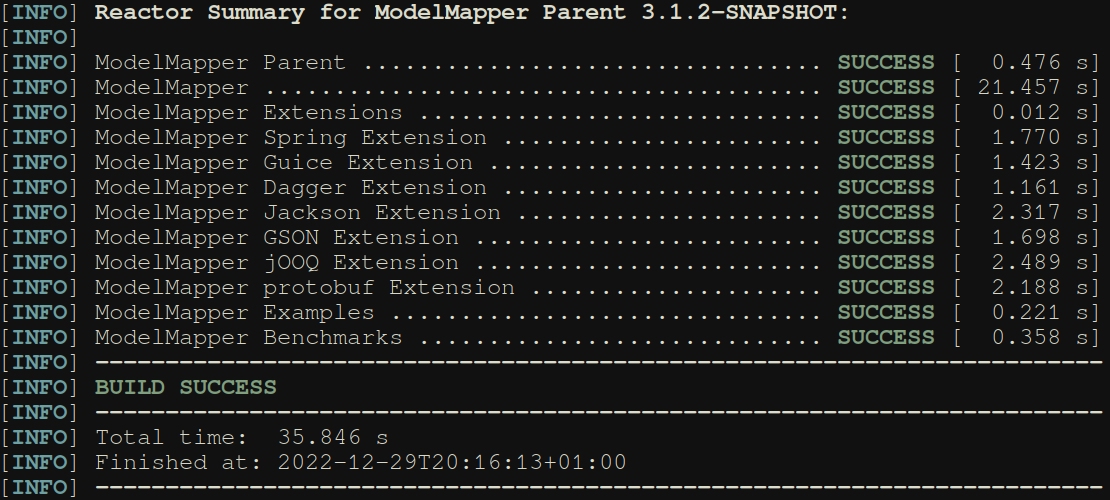
\includegraphics[width=14cm]{images/test-suite.png}
    \caption{Running the test suite from the terminal}
    \label{running-test-suite}
\end{figure}

\begin{figure}[H]
    \centering
    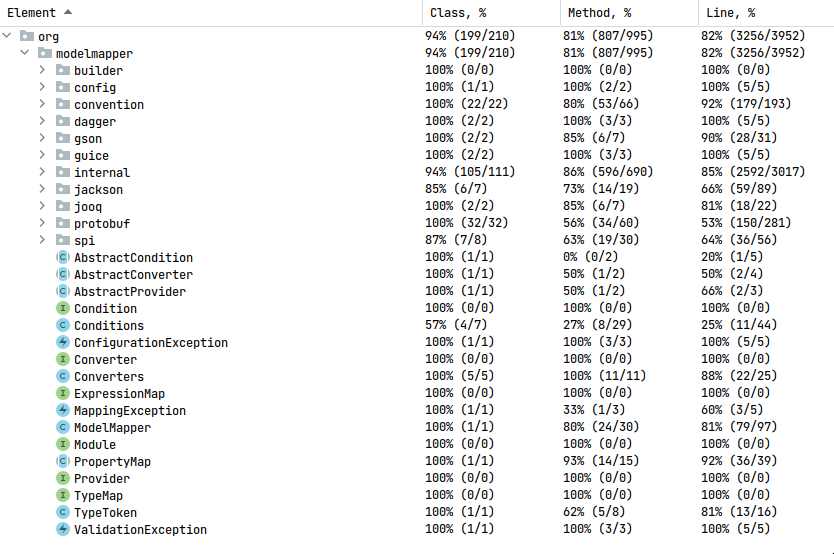
\includegraphics[width=14cm]{images/code-coverage.png}
    \caption{Code coverage metrics generated by IntelliJ}
    \label{intellij-code-coverage}
\end{figure}

Additionally, object-oriented data about the project was
extracted using CodeMR.

\begin{figure}[H]
    \centering
    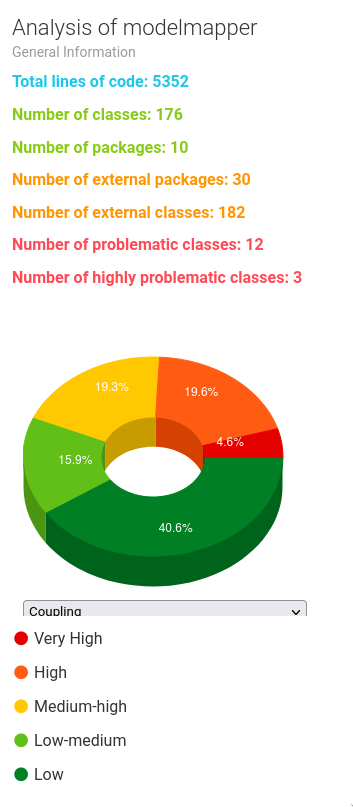
\includegraphics[height=12cm]{images/codemr-metrics.png}
    \caption{HTML report generate by CodeMR for the \modelmapper
    module}
    \label{codemr-metrics}
\end{figure}

\section{Project Analysis}

\subsection{Object--Oriented Metrics}

\subsubsection{Complexity}

\begin{figure}[H]
    \centering
    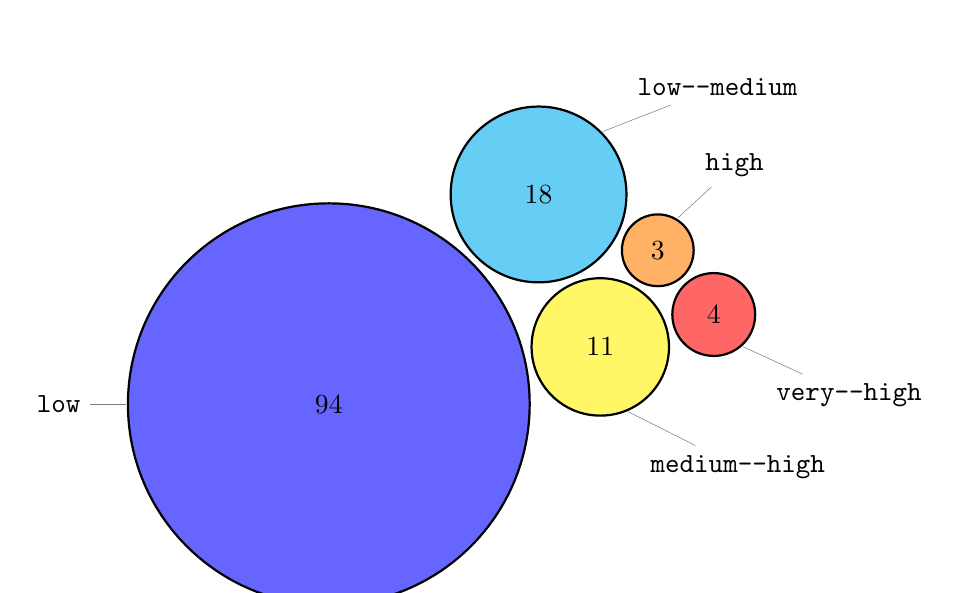
\begin{tikzpicture}
        \pie[sum=auto, cloud, text=pin]{
            94/\texttt{low},
            18/\texttt{low--medium},
            11/\texttt{medium--high},
            3/\texttt{high},
            4/\texttt{very--high}
        }
    \end{tikzpicture}
    \caption{Number of classes which have \texttt{low} to
    \texttt{very--high} complexity}
\end{figure}

\note{The percentage values provided by CodeMR were not used.
This is because when converting from percentages to quantities
the values were not identical to the ones reported by CodeMR.}

CodeMR defines code complexity in the following way.

\begin{definition}
    A class is said to be \ul{complex} if it is difficult to
    understand and describes the interactions between a number
    of entities. Higher levels of complexity increase the risk
    of unintentionally interfering with interactions and so
    increases the chance of introducing defects when making
    changes.
\end{definition}

CodeMR reports that only $7$ classes have a \texttt{high} or
\texttt{very--high} complexity. However, this does not mean that
the project is not complex.

Apart from the complexity brought on by \textbf{branching} as
mentioned in McCabe's Cyclomatic Complexity, there are other
factors. Specifically, \textbf{indirection} caused by dependency
injection or function calls also add complexity. This is because
a programmer has to jump from one segment of code to another to
understand.

\begin{figure}[H]
    \centering
    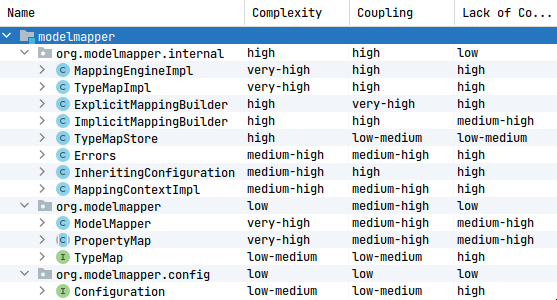
\includegraphics[width=14cm]{images/problematic-classes.png}
    \caption{The list of problematic classes identified by CodeMR}
    \label{problematic-classes}
\end{figure}

\begin{lstlisting}[language=Java,label={internal-method},caption={An
internal method in the class \texttt{TypeMapImpl} which
was reported by CodeMR as having \texttt{very--high}
complexity}]
@Override
public <P> TypeMap<S, D> include(TypeSafeSourceGetter<S, P> sourceGetter, Class<P> propertyType) {
  @SuppressWarnings("unchecked")
  TypeMapImpl<? super S, ? super D> childTypeMap = (TypeMapImpl<? super S, ? super D>)
      configuration.typeMapStore.get(propertyType, destinationType, name);
  Assert.notNull(childTypeMap, "Cannot find child TypeMap");

  List<Accessor> accessors = PropertyReferenceCollector.collect(this, sourceGetter);
  for (Mapping mapping : childTypeMap.getMappings()) {
    InternalMapping internalMapping = (InternalMapping) mapping;
    addMapping(internalMapping.createMergedCopy(accessors, Collections.<PropertyInfo>emptyList()));
  }
  return this;
}
\end{lstlisting}

Furthermore, additional barriers to understanding this
particular project are: extensive use of \textbf{unchecked
code}, \textbf{reflection} and \textbf{generics} (see listing
\ref{internal-method}). Unfortunately, Java has limited
capabilities when it comes to reflection and generics requiring
the use of unchecked code.

This naturally makes the project for any observer highly
complex. However, after acquainting one's self with the
terminology used and the less complex classes in the project, it
will overall be easier to understand the more complicated pieces
of code. Additionally, looking at the User Manual on
\url{https://modelmapper.org} will help in the understanding process.

Even though this system according to Lehman's Laws is very close
to an \texttt{S}--type system. Given the lack of
implementation--focused specification it makes the project more
complicated then it has to be. This is because individual
developer choices can heavily effect the complexity of the code.

So, from this perspective the project has a \textbf{medium}
complexity given that it is solving quite a complicated problem.
However, it might pose resitance to new contributors due to this
complexity. This can be easily remedied with more friendly and
implementation--focused specification.

\subsubsection{Coupling}

\begin{figure}[H]
    \centering
    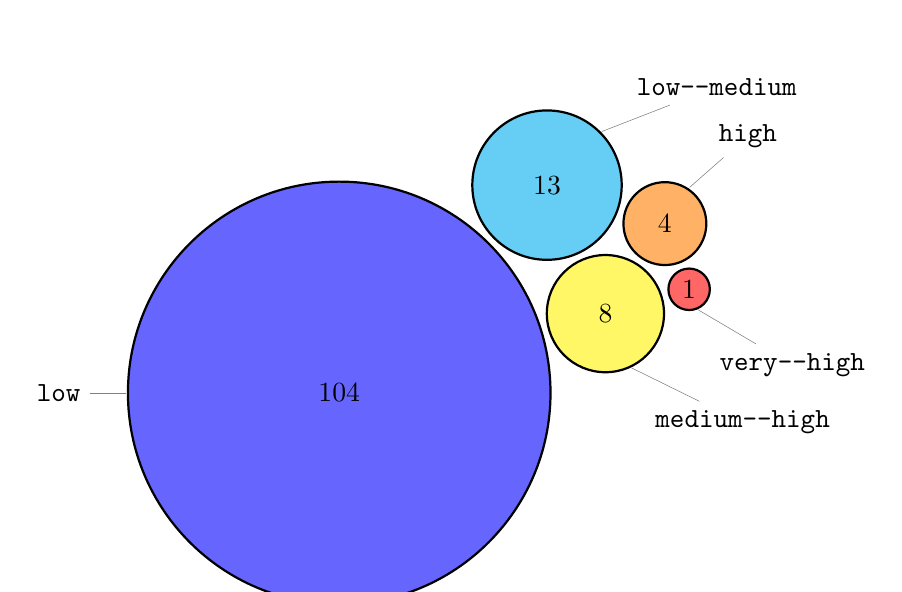
\begin{tikzpicture}
        \pie[sum=auto, text=pin, cloud]{
            104/\texttt{low},
            13/\texttt{low--medium},
            8/\texttt{medium--high},
            4/\texttt{high},
            1/\texttt{very--high}
        }
    \end{tikzpicture}
    \caption{Number of classes which have \texttt{low} to
    \texttt{very--high} coupling}
    \label{coupling-diag}
\end{figure}

\begin{definition}
    Two classes \textbf{A} and \textbf{B} are \ul{coupled} if:
    \begin{itemize}
        \item \textbf{A} has an attribute that refers to (is of type)
            \textbf{B}.
        \item \textbf{A} calls on services of an object
            \textbf{B}.
        \item \textbf{A} has a method that references \textbf{B}
            (via return type or parameter).
        \item \textbf{A} has a local variable which type is
            class \textbf{B}.
        \item \textbf{A} is a subclass of (or implements) class
            \textbf{B}.
    \end{itemize}

    Furthermore, tightly coupled systems tend to exhibit the
    following characteristics:
    \begin{itemize}
        \item A change in a class usually forces a ripple effect
            of changes in other classes.
        \item Requires more effort and/or time due to the
            increased dependency.
        \item Might be harder to reuse a class because dependent
            classes must be included.
    \end{itemize}
\end{definition}

As can be seen in figure \ref{problematic-classes}, there are
$5$ problematic classes (also mentioned in figure
\ref{coupling-diag}) which have been marked as having high
coupling.

\begin{figure}[H]
    \centering
    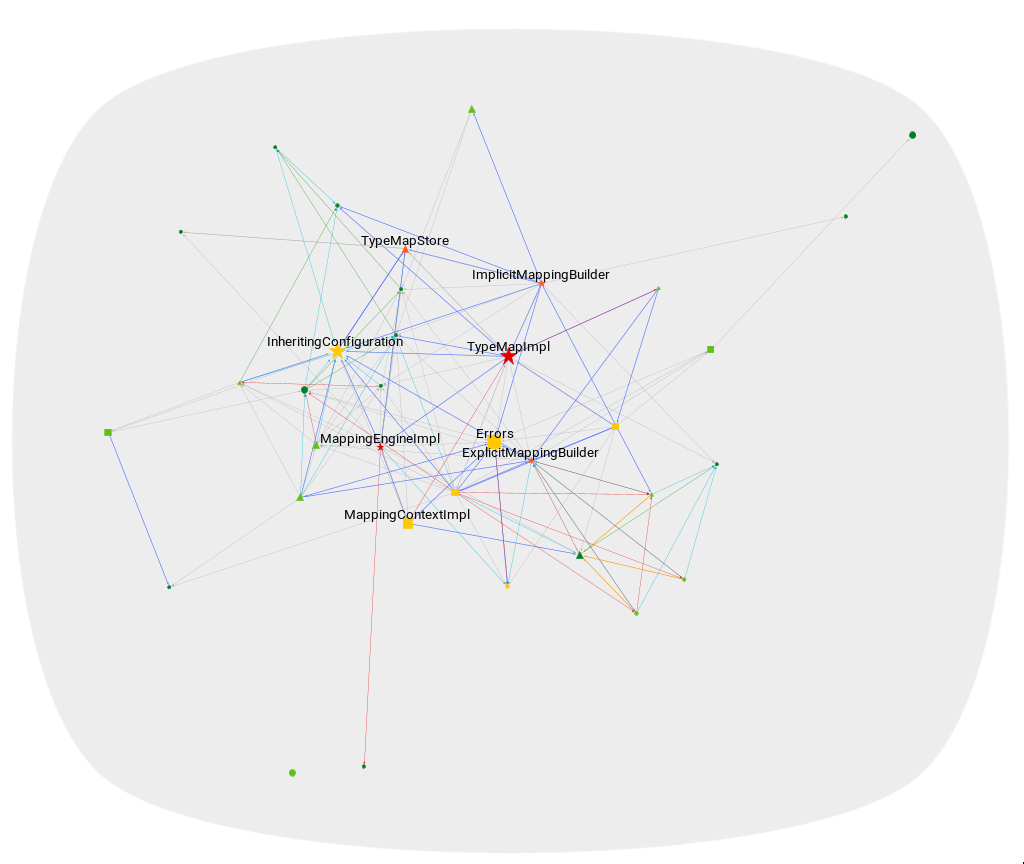
\includegraphics[width=16cm]{images/internal-package-coupling.png}
    \caption{A dependency graph of all the classes in the
    \texttt{org.modelmapper.interal} package generated by
    CodeMR}
    \label{internal-package-coupling}
\end{figure}

Clearly, these classes seem to be doing most of the heavy
lifting, in fact most of the complexity is also present in these
classes. So as consequence high coupling is expected. This is
clear in the dependency visualisation in figure
\ref{internal-package-coupling}. Also, the type of coupling
present between classes is \emph{Common Coupling}. This is
because the classes have instances of each other present as
class fields and they share a lot of data and configuration.

\note{This coupling is not happening at a package level but at a
class level. This makes it a less severe form of coupling.
However, it still hinders understandability.}

As a suggestion, to reduce coupling (and even complexity) a more
structured approach to dependency management should be taken. If
necessary, even having code duplication to allow for decoupling
would be better as it isolates all the dependencies required by
a specific class. Ideally, the dependency graph should look like
a tree.

\subsubsection{Cohesion}

\begin{figure}[H]
    \centering
    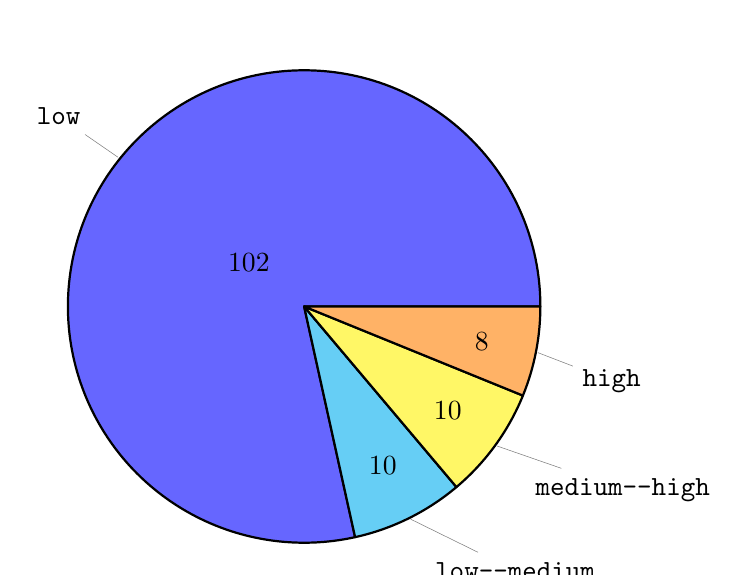
\begin{tikzpicture}
        \pie[sum=auto, text=pin]{
            102/\texttt{low},
            10/\texttt{low--medium},
            10/\texttt{medium--high},
            8/\texttt{high}
        }
    \end{tikzpicture}
    \caption{Number of classes which have \texttt{low} to
    \texttt{high} \textbf{lack of cohesion}}
    \label{cohesion-diag}
\end{figure}

\begin{definition}
    \ul{Cohesion} is a measure of how well the methods of
    a class are related to each other. High cohesion (low lack
    of cohesion) tend to be preferable, because high cohesion is
    associated with several desirable traits of software
    including robustness, reliability, reusability, and
    understandability. In contrast, low cohesion is associated
    with undesirable traits such as being difficult to maintain,
    test, reuse, or even understand.
\end{definition}

As can be seen in figure \ref{cohesion-diag} there are no classes
which have a very high lack of cohesion. Nevertheless, there are
some which have high lack of cohesion. Again looking at
figure \ref{problematic-classes}, they are essentially, the same
classes described in the prior section.

Closer inspection of the actual classes reveals that these,
where possible, are following a form of cohesion called
\emph{Procedural Cohesion} or they expose their methods to their
consumers.

Procedural Cohesion is a type of cohesion where methods are
grouped together because they form part of a chain of execution.

Cohesion can be improved by trying to break the code into
methods which can be reused in multiple places in the class.
However, of course this is not always possible.

\subsection{Test Suite Suitability}

The overall line coverage of the project was $82\%$. This is a
significant amount of the code and hence the project is being
sufficiently tested with regards to all possible code paths.

Nevertheless, this is \textbf{not} a guarantee of the project's
quality. This is because certain tests can have artificially
high code coverage whilst only really testing a small subset of
the covered area. This is very common when unit tests call
high--level methods to test the library/application.

\begin{figure}[H]
    \centering
    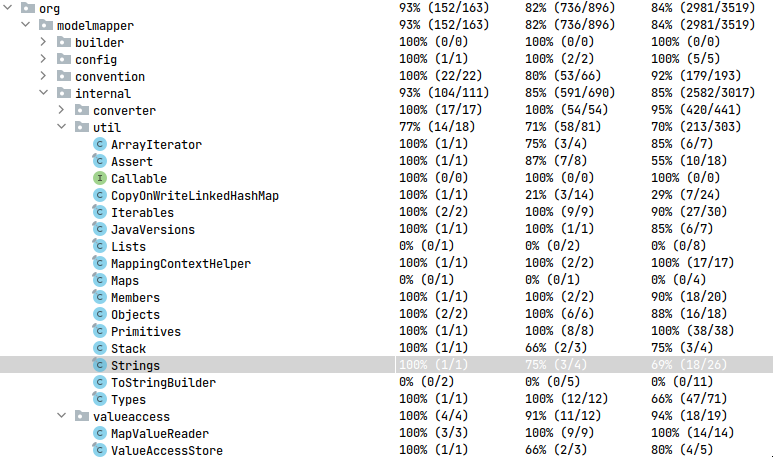
\includegraphics[width=14cm]{images/code-coverage-2.png}
    \caption{Further code coverage metrics generated by IntelliJ}
    \label{intellij-code-coverage-2}
\end{figure}

Overall the project has enough unit tests however there are
some gaps. Going over the code the following observations can be
made:

\begin{itemize}
    \item Getters are often ignore and not tested. Presumably,
        because they are very simple.
    \item Catch blocks also seem to be minimally tested.
    \item Some classes are not covered at all for example
        \texttt{BridgeClassLoaderFactory}, \linebreak
        \texttt{StrongTypeConditionalConverter} etc.
    \item Some classes also seem to be partially covered as a side
        effect of some other test for example
        \texttt{CopyOnWriteLinkedHashMap}.
\end{itemize}

Now, if we take into consideration the data generated by CodeMR
(see figure \ref{problematic-classes}), there is a large
concentration of tests focused on testing the packages with the
most complex classes (see figure
\ref{intellij-code-coverage-2}). The package in question is
\texttt{org.modelmapper.internal} and it is has a coverage of
around $85\%$.

\subsection{Maintainability}

\subsubsection{Development Cycle}

\begin{figure}[H]
    \centering
    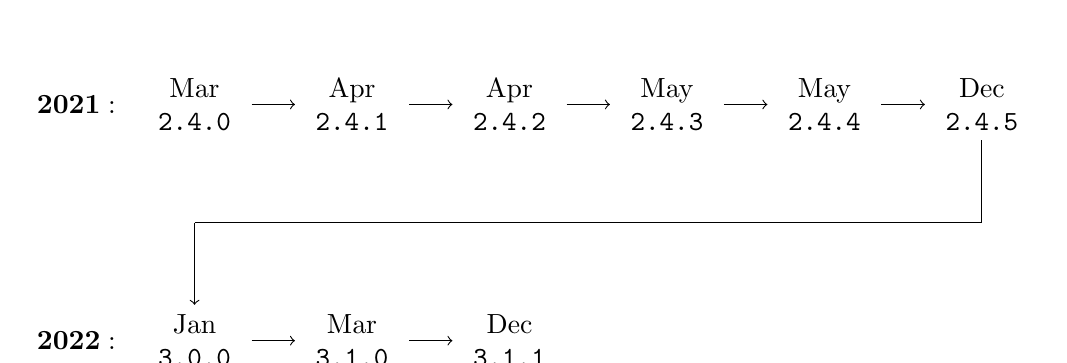
\begin{tikzpicture}
        \node (year2021) at (-1.5,3) {$\mathbf{2021:}$};
        \node (year2022) at (-1.5,0) {$\mathbf{2022:}$};

        \node[text width=1.2cm, align=center] (A) at (0,3)  {Mar \texttt{2.4.0}};
        \node[text width=1.2cm, align=center] (B) at (2,3)  {Apr \texttt{2.4.1}};
        \node[text width=1.2cm, align=center] (C) at (4,3)  {Apr \texttt{2.4.2}};
        \node[text width=1.2cm, align=center] (D) at (6,3)  {May \texttt{2.4.3}};
        \node[text width=1.2cm, align=center] (E) at (8,3)  {May \texttt{2.4.4}};
        \node[text width=1.2cm, align=center] (F) at (10,3) {Dec \texttt{2.4.5}};
        \node[text width=1.2cm, align=center] (G) at (0,0)  {Jan \texttt{3.0.0}};
        \node[text width=1.2cm, align=center] (H) at (2,0)  {Mar \texttt{3.1.0}};
        \node[text width=1.2cm, align=center] (I) at (4,0)  {Dec \texttt{3.1.1}};

        \coordinate (left) at (0, 1.5);
        \coordinate (right) at (10, 1.5);

        \draw[->] (A) -- (B);
        \draw[->] (B) -- (C);
        \draw[->] (C) -- (D);
        \draw[->] (D) -- (E);
        \draw[->] (E) -- (F);
        \draw (F) -- (right);
        \draw (right) -- (left);
        \draw[->] (left) -- (G);
        \draw[->] (G) -- (H);
        \draw[->] (H) -- (I);
    \end{tikzpicture}
    \caption{Project releases in the past two years ($2021$ and
    $2022$)}
    \label{project-releases}
\end{figure}

The development cycle does not seem to follow any predefined
schedule. In fact in the year $2021$ there were twice as many
releases as in the year $2022$. Also, in previous years there
was more signigificant activity. In general, releases used to
contain a decent amount of work. In these last two years work on
the project seems to have slowed down.

\subsubsection{Commit Analysis}

The following ten commits were analysed:

\begin{enumerate}
    \item Add error message while skip conflict
        (\texttt{00a45001a73ee65f4351b48f97bb083cc2ae0d6e})
    \item Add unit tests for optional converters
        (\texttt{4b3cc868aacbc797ee2433c77938d62d6e62692d})
    \item Improve performance on implicit mapping (\#$619$)
        \newline
        (\texttt{2f5b7ccca0e56c7d529e6626b43746e583824910})
    \item Fix logical bug in PropertyInfoRegistry
        (\texttt{9ab5eaacfaf2cd3fb0c079346a6c205317122a49})
    \item Fix configuration `collectionsMergeEnabled',
        `deepCopyEnabled' (\#$485$) \newline
        (\texttt{b77316ba99ec52b1c497280a31da19ef0c29eedf}) 
    \item Change collections merge strategy breaks mapping of
        collection from a\ldots \newline
        (\texttt{6606f3d16b127c1577b7555402954d0aca33ceeb})
    \item Parse date from String to java.util.Date in yyyy-MM-dd
        format \newline
        (\texttt{8a69be1a65f0abc05f19f2add81e95e36bed696c})
    \item In order to use ModelMapper in jdk11 (build 11+28).
        \newline
        (\texttt{096183809417d0ff65b2f09c7995913cf877a54f})
    \item Fixes MapValueReader get wrong field type (\#$371$)
        \newline
        (\texttt{fbc99db5785bdc51b3a896dbf7442e83c7ac95c5}) 
    \item Updates asm, cglib and objenesis to their latest
        versions \newline
        (\texttt{d66343ed9eb10d91220baa0a5a2a4be66e212ae3})
\end{enumerate}

\begin{figure}[H]
    \centering
    
\includegraphics[width=14cm]{images/pull-request.png}
    \caption{Pull request associated with the \nth{6} commit}
    \label{pull-request}
\end{figure}

In terms of readability, it depends which commit one considers.
This is because some commits are inherintely very simple. For
example the \nth{10} commit is a perfective commit; just bumping
the versions of the described dependencies in the
\texttt{pom.xml} file. Also, there are commits coming from pull
requests which are corrective in nature that are also very well
explained by the author (see figure \ref{pull-request}).

However, there are commits from the core maintainers of the
repository which are not very well explained. This is a symptom
of having extensive knowledge of the project. To core
maintainers many parts of the project might seem simple whereas,
to new maintainers they might not be so simple. Of course some
initial investment to acclimate to the project is still
required.

Open--source projects suffer the same cost of onboarding new
developer as For--profit companies, but to a greater extent
since there is often no monetary motivater.

In previous yreas ($2018$--$2020$) the project was much more
active. There was significant activity on GitHub and in each
development cycle it was more common for the core maintainers to
merge pull--requests submitted by contributors. Additionally,
the core maintainers would also help contributors by reviewing
code and providing suggestions to improve code (see the \nth{10}
commit).

Pull requests and issues were significantly used and were a
good measure of the amount of work being done. Additionally, the
core maintainers also adopted a system of calling certain test
classes \verb|GH{issue-number}|, where \texttt{GH} stands for
GitHub to directly link the class to a GitHub issue or bug
where most of the discussion and exposition for the bug would be
stored.

Additionally, GitHub provides features for more explicit planning
and development of certain features however, it is very likely
that the core maintainers believe that the library itself is
feature complete and does not need additional changes, except
for maintenance and new features added by contributors.

\subsubsection{Analysing Commit
\texttt{00a45001a73ee65f4351b48f97bb083cc2ae0d6e}}

\begin{figure}[H]
    \centering
    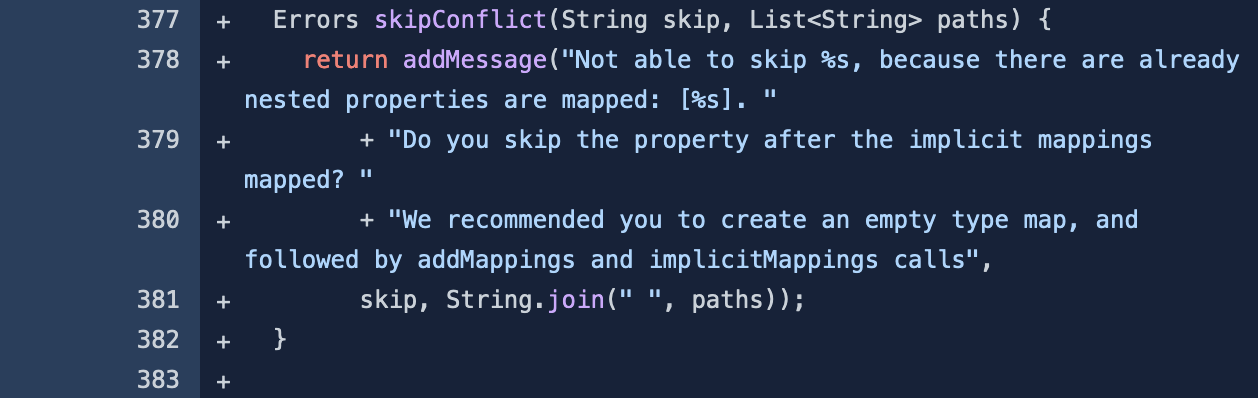
\includegraphics[width=14cm]{images/code-diff.png}
    \caption{Addition of a new error message in
    \texttt{Errors.java}}
    \label{error-message}
\end{figure}

The above commit hash refers to the first commit in our list of
analysis. Specifically, ``Add error message while skip
conflict''. This commit falls under the category of perfective
maintenance. This is because the core maintainer is adding an
additional error message (see figure \ref{error-message}) meant
to aid users and help users understand how \modelmapper is
supposed to work.

The core maintainer decided to add this commit after a number of
users commented on
\href{https://github.com/modelmapper/modelmapper/issues/633}{GitHub
issue 633} and
\href{https://github.com/modelmapper/modelmapper/issues/654}{GitHub
issue 654} about some expected behvaiour. The expected behaviour
by the users was that the nested fields of internal object where
also skipped. However, this was not the case.

Additionally, the maintainer also added a test class called
\texttt{GH654.java} in the \linebreak \texttt{org.modelmapper.bugs} package
to make sure that the behaviour is properly documented.

\note{At the time of writing both issue 633 and 654 were open.}

\end{document}
